%% Características del switch principal del GRID

\begin{table}[H]
	\centering
	\sffamily\scriptsize
	\setlength{\tabcolsep}{4pt}
	\renewcommand{\arraystretch}{1.3}
	\caption{Ficha técnica --- Switch Cisco SG200-26}
	\label{table:big-switch}
	\begin{tabular}{|p{0.25\textwidth}|p{0.6\textwidth}|p{0.12\textwidth}|}
		\hline
		\rowcolor{gray!15} \multicolumn{3}{|c|}{\textbf{DESCRIPCIÓN FÍSICA:} Switch administrable de 26 puertos}                                                                                                                                 \\ \hline

		\textbf{TIPO DE RECURSO:}                     & Switch Gigabit administrable & \multirow{3}{*}{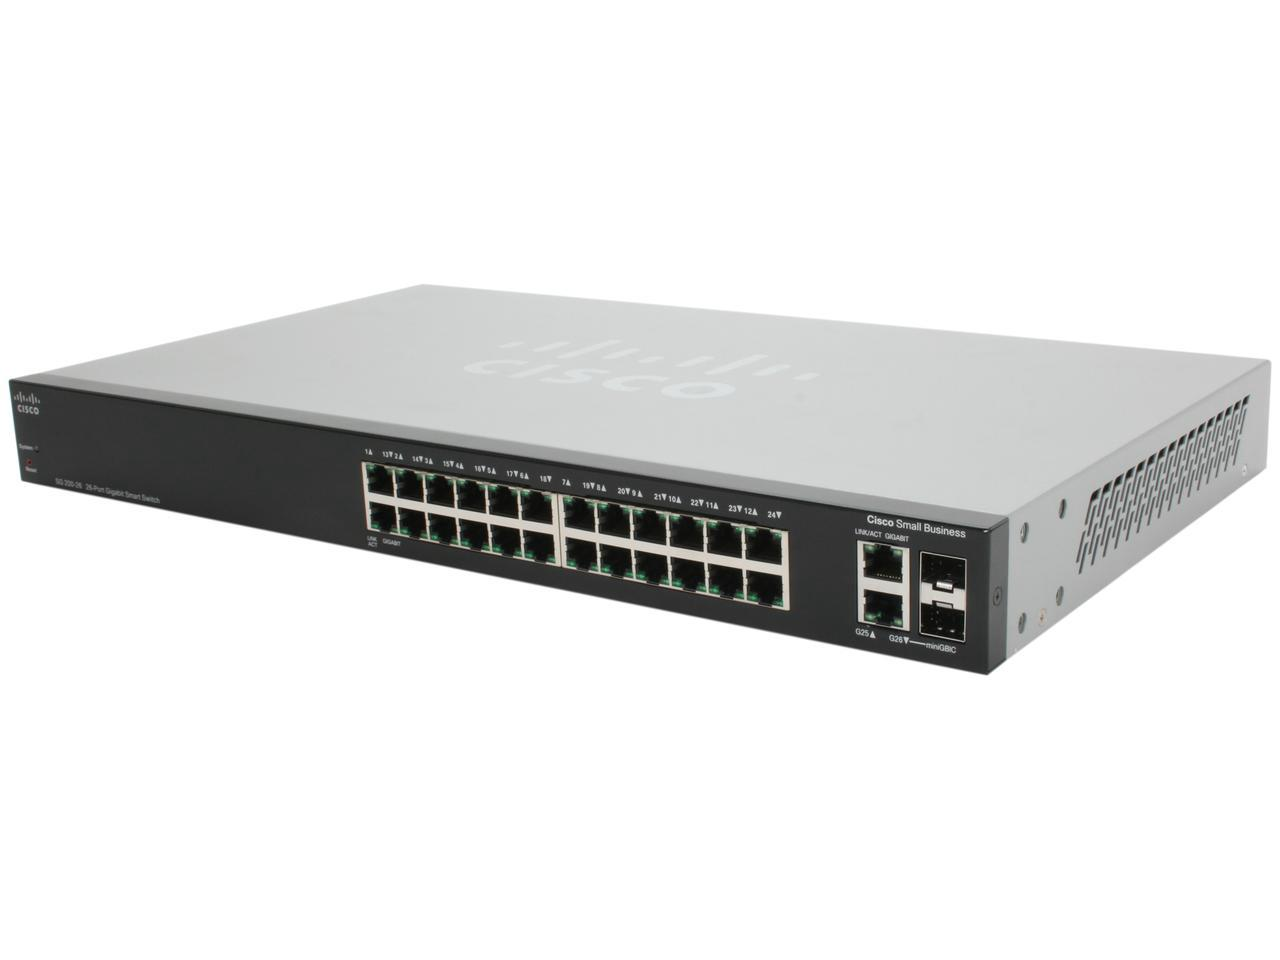
\includegraphics[width=\linewidth,keepaspectratio]{tablas-images/raspberries/big-switch.jpg}}                                             \\ \cline{1-2}
		\textbf{MODELO:}                              & SG200-26                     &                                                                                                                                                           \\ \cline{1-2}
		\textbf{MARCA:}                               & Cisco                        &                                                                                                                                                           \\ \hline

		\rowcolor{gray!15} \multicolumn{3}{|c|}{\textbf{ESPECIFICACIONES TÉCNICAS}}                                                                                                                                                              \\ \hline

		\textbf{Rendimiento}                          &
		\begin{minipage}[t]{\linewidth}
			\vspace{2pt}
			• Capacidad de Conmutación: 52 Gbps \\
			• Capacidad de Reenvío: 38.69 Mpps \\
			• Tabla de direcciones MAC: 8,000 entradas \\
			• Jumbo Frames: Soportado
			\vspace{2pt}
		\end{minipage} &                                                                                                                                                                                               \\ \hline

		\textbf{Interfaces}                           &
		\begin{minipage}[t]{\linewidth}
			\vspace{2pt}
			• 24 puertos RJ-45 10/100/1000 Mbps \\
			• 2 puertos combo Gigabit SFP \\
			• Auto-negociación y auto-MDI/MDIX \\
			• Soporte IEEE 802.3ad (Link Aggregation)
			\vspace{2pt}
		\end{minipage}     &                                                                                                                                                                                                 \\ \hline

		\textbf{Administración}                       &
		\begin{minipage}[t]{\linewidth}
			\vspace{2pt}
			• Interfaz web de administración \\
			• SNMP, RMON, HTTP, TFTP \\
			• Cisco Discovery Protocol \\
			• Auto SmartPorts \\
			• Soporte DHCP y BOOTP
			\vspace{2pt}
		\end{minipage}           &                                                                                                                                                                                                         \\ \hline

		\textbf{Características Avanzadas}            &
		\begin{minipage}[t]{\linewidth}
			\vspace{2pt}
			• VLAN support (IEEE 802.1Q) \\
			• Quality of Service (QoS) \\
			• IGMP/MLD Snooping \\
			• Spanning Tree (STP/RSTP) \\
			• IEEE 802.1x Authentication \\
			• Storm Control (Broadcast/Multicast/Unicast)
			\vspace{2pt}
		\end{minipage} &                                                                                                                                                                                             \\ \hline

		\textbf{Características Físicas}              &
		\begin{minipage}[t]{\linewidth}
			\vspace{2pt}
			• Alimentación: 100-240V AC, 50-60 Hz \\
			• Dimensiones: 439 × 257 × 43 mm \\
			• Peso: 3.3 kg (7.2 lbs) \\
			• Montaje: Rack 1U \\
			• Diseño sin ventiladores
			\vspace{2pt}
		\end{minipage}      &                                                                                                                                                                                                    \\ \hline

		\textbf{Memoria y Estándares}                 &
		\begin{minipage}[t]{\linewidth}
			\vspace{2pt}
			• Flash: 16 MB, RAM: 128 MB \\
			• IEEE 802.3/802.3u/802.3z/802.3ab \\
			• Certificaciones: UL 60950, FCC Part 15A \\
			• MTBF: 194,278 horas
			\vspace{2pt}
		\end{minipage}  &                                                                                                                                                                                                \\ \hline

		\rowcolor{gray!15} \multicolumn{3}{|l|}{\textbf{PROPÓSITO:} Switch unifica las conexiones del clúster HTCondor}                                                                                                                          \\ \hline
		\multicolumn{3}{|p{0.97\textwidth}|}{\textbf{OBSERVACIONES:} Switch administrable de nivel empresarial que proporciona conectividad Gigabit con funciones avanzadas de gestión, VLAN, QoS y seguridad para la infraestructura del GRID.} \\ \hline
	\end{tabular}
\end{table}
